\section{Systemmodelle}
% TODO T Nummern anpassen

\subsection{Globale Testfälle}
Folgende Funktionssequenzen sind zu überprüfen:

\begin{itemize}
\item /T110/ Erstmaliges Starten des Programms
\begin{itemize}
\item Während das Programm sich im Ladebildschirm befindet, werden dem Spieler Comic-artige Sprechbblasen mit lustigen und interessanten Texten angezeigt.
\item Der Nutzer startet das Programm und befindet sich im Menü "`Sprachauswahl"'. Mit den Knöpfen TODO und TODO wählt er seine Sprache aus.
\item Durch Drücken des Knopfes TODO wechselt das Programm zum Menü "`Namenseingabe"'. Hier wird der Spieler nach seinem Namen gefragt, den er in der Textbox eingibt.
\item Durch Drücken des Knopfes TODO wechselt das Programm zum Menü "`Avatarauswahl"'. Mit den Knöpfen TODO und TODO wählt er den gewünschten Avatar aus.
\item Durch Drücken des Knopfes TODO erscheint der Begrüßungsbildschirm mit Name und Avatar des Spielers.
\item Nach 3 Sekunden wechselt das Programm automatisch zum Hauptmenü.
\end{itemize}

\item /T120/ Starten des Programms, nachdem mindestens ein Profil bereits erstellt wurde
\begin{itemize}
\item Der Nutzer startet das Programm und befindet sich im Menü "`Profilauswahl"'. Hier wählt er durch Drücken des Knopfes TODO mit seinem Namen sein Profil aus.
\item Durch Drücken des Knopfes TODO erscheint der Begrüßungsbildschirm mit Name und Avatar des Spielers.
\item Nach 3 Sekunden wechselt das Programm automatisch zum Hauptmenü.
\end{itemize}

\item /T130/ Profildaten ändern
\begin{itemize}
\item Der Nutzer befindet sich im Hauptmenü und drückt auf den Knopf TODO. Das Programm wechselt zum Optionsmenü.
% Knopf "Profil editieren"
\item Durch Drücken des Knopfes TODO wechselt das Programm zum Menü "`Sprachauswahl"'. Wie in /T110/ beschrieben gibt der Nutzer nacheinander Sprache, Namen und Avatar ein.
\item Nach Drücken des Knopfes TODO im Menü "`Avatarauswahl"' wechselt das Programm zurück in das Optionsmenü.
\end{itemize}

\item /T140/ Profil löschen
\begin{itemize}
\item Der Nutzer befindet sich im Hauptmenü und drückt auf den Knopf TODO. Das Programm wechselt zum Optionsmenü.
% Knopf "Profil löschen"
\item Durch Drücken des Knopfes TODO öffnet sich ein Popupfenster, in dem das Löschen bestätigt wird.
\item Nach Bestätigung wechselt das Programm zum Menü "`Profilauswahl"'. Das Profil ist jetzt gelöscht und hier nicht mehr auswählbar.
\end{itemize}

\item /T150/ Einen Term im Editor-Modus bearbeiten
\begin{itemize}
\item Der Nutzer hat ein Level gestartet und befindet sich jetzt im Editor-Modus.
% Knops "Hinweis"
\item Durch Drücken des Knopfes TODO öffnet sich ein Popupfenster, in welchem dem Spieler ein Hinweis zur Lösung des aktuellen Levels gegeben wird.
\item Durch die Drag\&Drop Geste fügt er nacheinander sowohl ein weißes Lamm als auch ein weißer Edelstein zum aktuellen Term hinzu.
\item Durch Drücken des Lamms öffnet sich ein Kontextmenü, in dem der Spieler eine Farbe auswählen kann. Nach Drücken der gewünschten Option wechselt das Lamm seine Farbe.
\item Durch die Drag\&Drop Geste zum Werkzeugmenü entfernt der Spieler einen Edelstein aus dem Term.
\item Der Spieler versucht ein durch das Level bereits vorgegebenes Lamm durch die Drag\&Drop Geste zu verschieben, das Programm unterdrückt dies aber.
% Knopf "Play"
\item Der Term ist jetzt gültig und der Spieler drüct den Knopf TODO. Das Programm wechselt zum Reduktions-Modus.
\end{itemize}

\item /T150/ Einen Term im Reduktions-Modus konvertieren
\begin{itemize}
% Knopf "Play"
\item Der Nutzer hat nach Bearbeiten eines Terms im Editor-Modus den Knopf TODO betätigt und befindet sich jetzt im Reduktions-Modus.
% Knopf "Step forward"
\item Durch Drücken des Knopfes TODO wird der Term um einen Schritt reduziert.
% Knopf "Step backward"
\item Durch Drücken des Knopfes TODO wird der Term auf den Zustand vor dem letzten Schritt zurückgesetzt.
% Knopf "Play" "Pause"
\item Durch Drücken des Knopfes TODO werden automatisch einzelne Reduktionen nacheinander ausgeführt. Nach 3 Schritten drückt der Spieler den Knopf TODO und die Ausführung pausiert.
% Knopf "Step forward"
\item Durch Drücken des Knopfes TODO wird der Term um einen Schritt reduziert. Der Term ist jetzt minimal und gleich dem gewünschten Term, der durch das Level vorgegeben ist.
\item Ein Popup-Fenster wird geöffnet, in dem der Spieler darüber informiert wird, dass er das Level abgeschlossen hat.
\end{itemize}

\item /T160/ Level auswählen
\begin{itemize}
% Knopf "Level"
\item Der Nutzer befindet sich im Hauptmenü und drückt den Knopf TODO. Das Programm wechselt zum Menü "`Levelauswahl"'.
\item Einige Level sind bereits abgeschlossen und durch einen Haken markiert, ein Level ist freigeschaltet und die restlichen Level nicht freigeschaltet und durch ein Schloss markiert. Level mit demselben Schwierigkeitsgrad sind farblich gleich gekennzeichnet.
\item Der Spieler wählt ein Level aus und das Programm wechselt in den Editor-Modus zur Bearbeitung dieses Levels.
\end{itemize}

\item /T170/ Den Shop benutzen
\begin{itemize}
\item Nach erstmaligem erfolgreichen Abschließen eines Levels wird dem Spieler eine Anzahl von Münzen gutgeschrieben.
% Knopf "Shop"
\item Der Spieler befindet sich im Hauptmenü. Durch Drücken des Knopfes TODO wechselt er zum Menü "`Shop"'.
\item Hier wählt er den Menüpunkt "`Sounds"' aus. Es erscheinen mehrere zum Kauf verfügbare Objekte.
\item Der Spieler wählt einen Sound aus und wird darauf durch ein Popupfenster zur Bestätigung des Kaufs gebeten.
\item Nach der Bestätigung wird der Sound freigeschaltet und automatisch aktiviert.
\item Der Spieler aktiviert einen anderen Sound, indem er auf das entsprechende Element drückt. Das aktivierte Element wird durch einen Haken gekennzeichnet, der Haken beim deaktivierten Element wird entfernt.
\end{itemize}

\item /T180/ Optionen auswählen
\begin{itemize}
% Knopf "Toggle Music"
\item Das Programm befindet sich im Hauptmenü. Durch Drücken des Knopfes TODO wird die Hintergrundmusik deaktiviert.
% Knopf "Optionen" "Checkbox Lehrermodus"
\item Durch Drücken des Knopfes TODO wechselt das Programm in das Optionsmenü. Hier aktiviert der Spieler durch Drücken des Kontrollkästchens TODO den Lehrermodus.
% Knopf "Zurück"
\item Durch Drücken des Knopfes TODO wechselt das Programm zurück in das Hauptmenü.
\end{itemize}

\item /T190/ Benutzerstatistik ansehen
\begin{itemize}
% Knopf "Optionen"
\item Das Programm befindet sich im Hauptmenü. Durch Drücken des Knopfes TODO wechselt das Programm in das Optionsmenü.
% Knopf "Statistik"
\item Durch Drücken des Knopfes TODO wechselt das Programm in das Menü "`Statistik"'. Hier kann der Spieler verschiedene Daten zu seinem Spielverhalten einsehen.
% Knopf "Zurück"
\item Durch Drücken des Knopfes TODO wechselt das Programm zurück in das Optionsmenü.
\end{itemize}

\end{itemize}

\subsection{Datenkonsistenzen}

\begin{itemize}
\item /T210/ Ein Profil ist eindeutig durch den Namen gekennzeichnet. Es kann nicht mehrere Profile mit demselben Namen geben.
\end{itemize}

\subsection{Objektmodell}
% UML Klassendiagramme

\begin{figure}[H]
\centering
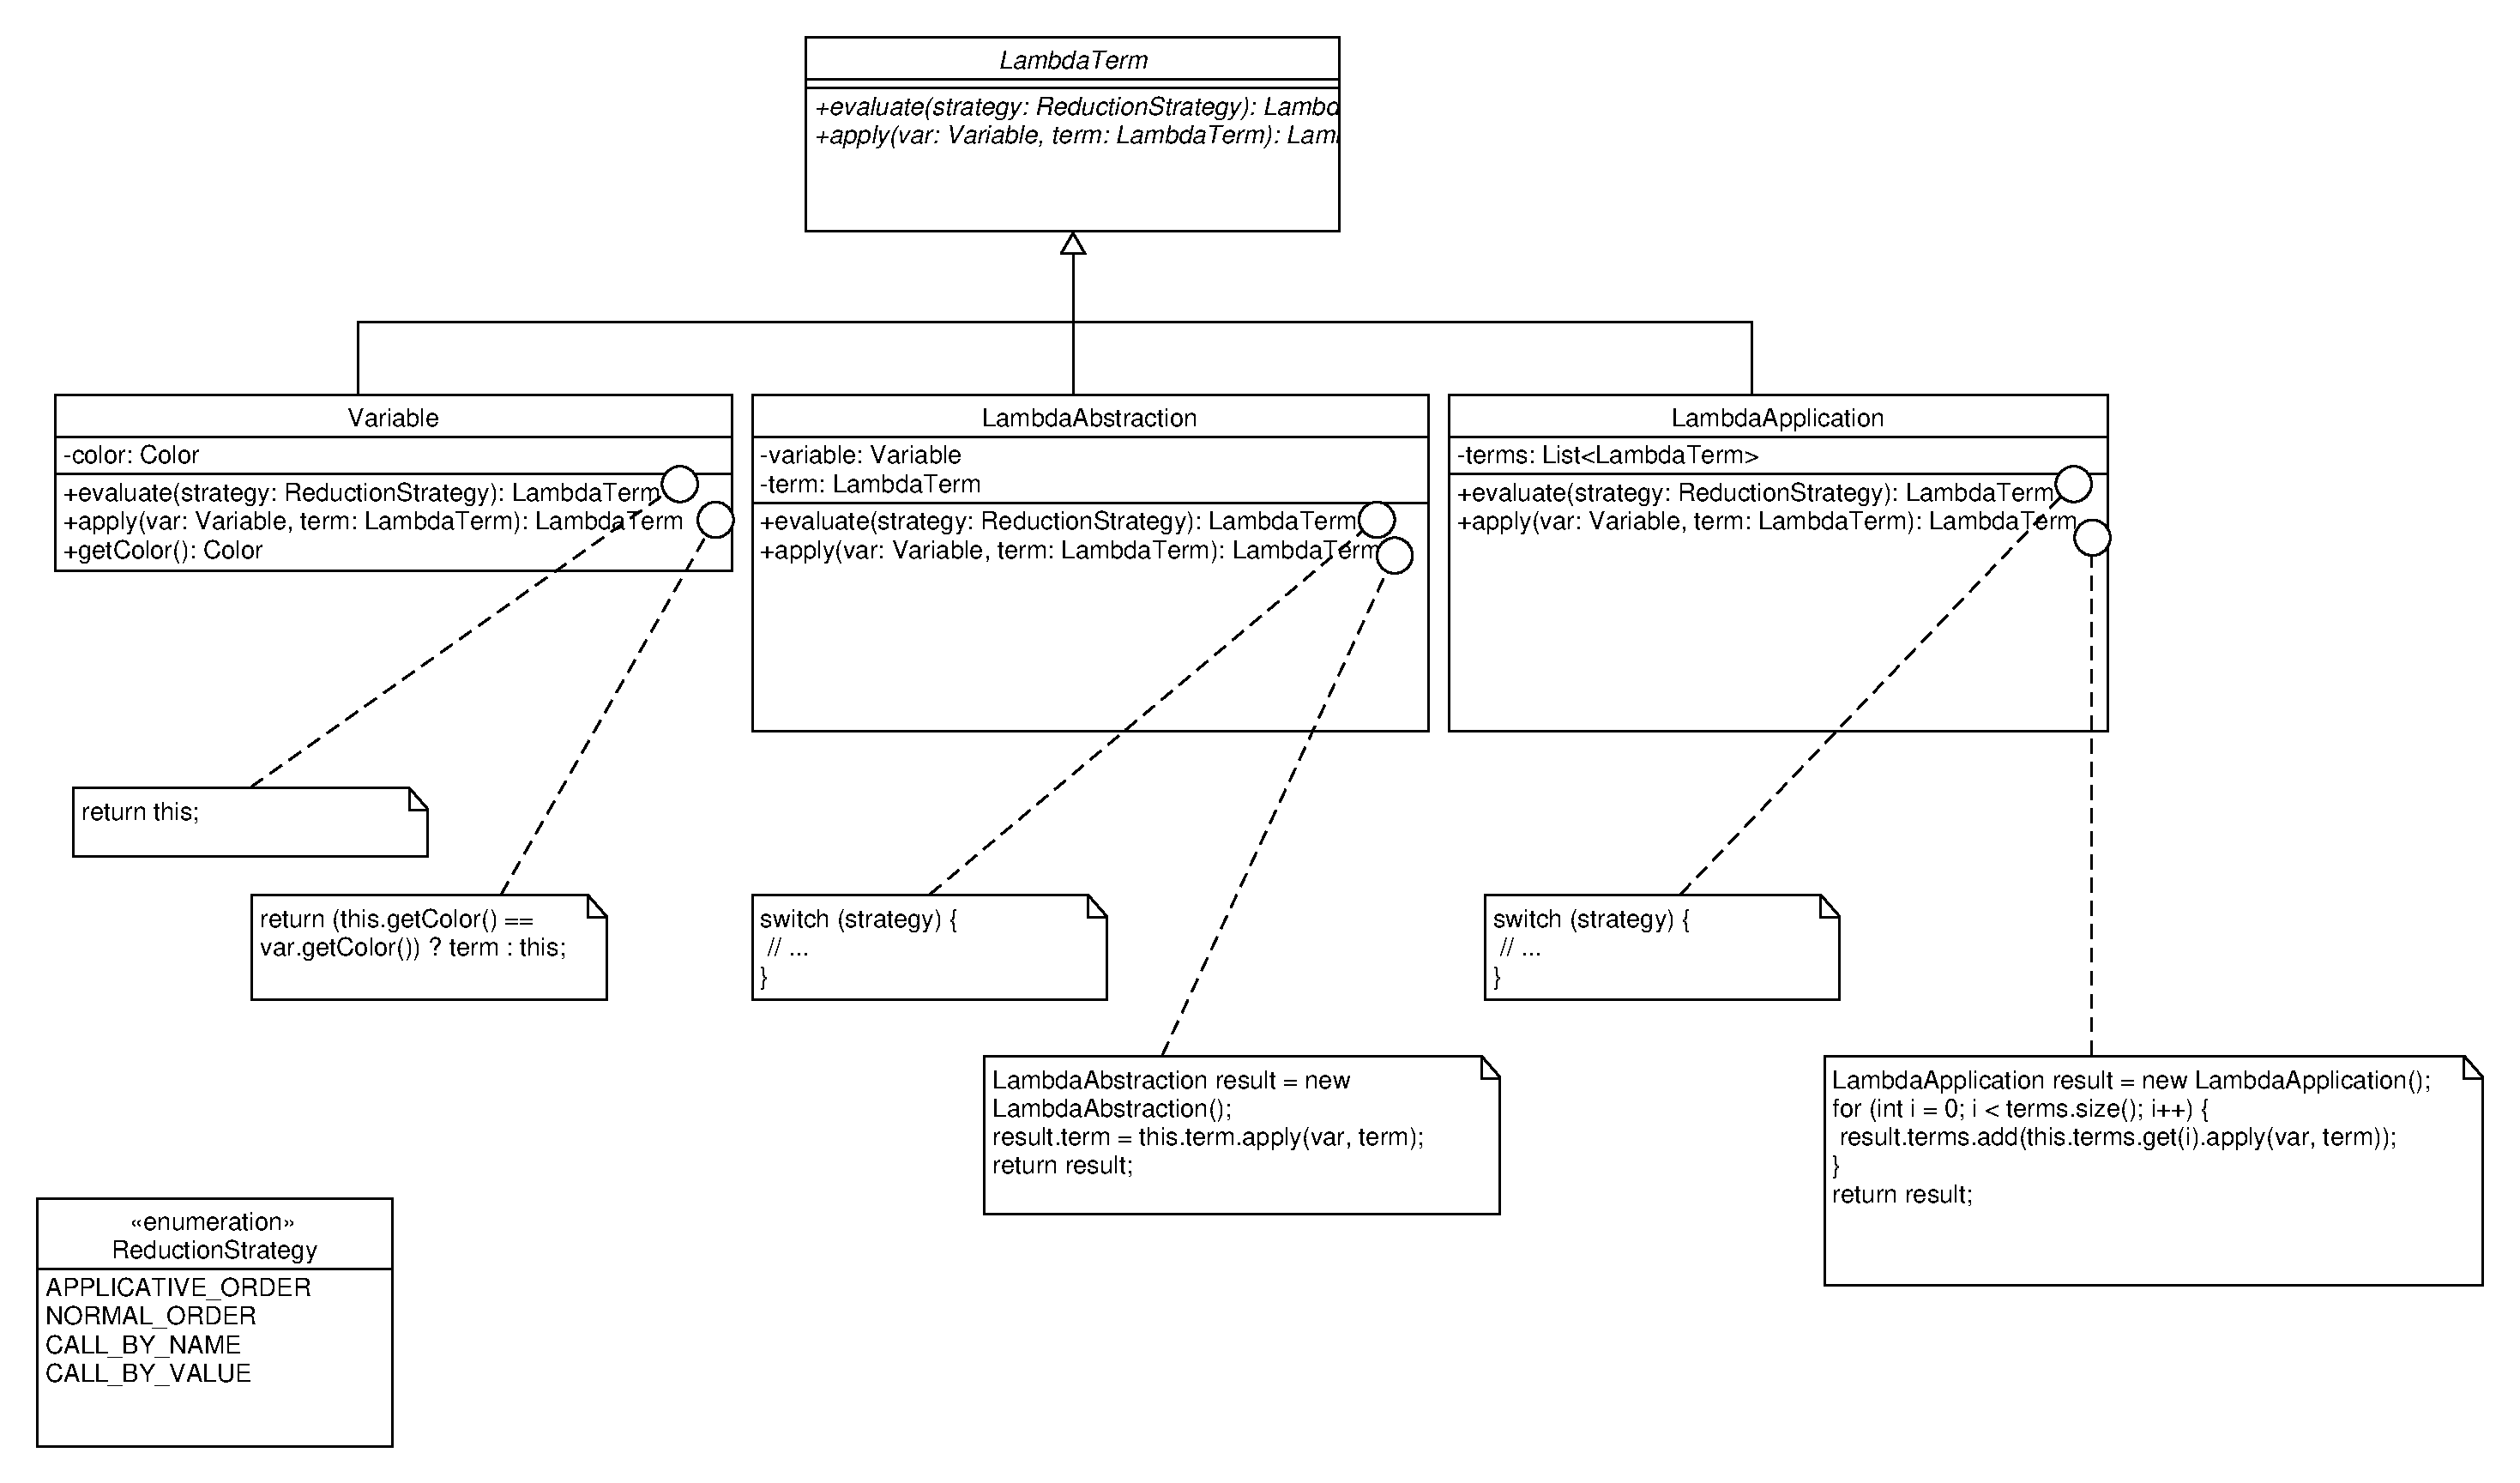
\includegraphics[scale=0.5]{../system_models/object_models/lambda_calculus.pdf}
\caption{UML Klassendiagramm zum Lambda-Kalkül}
\end{figure}

\subsection{Dynamische Modelle}
% UML Zustandsautomat, Sequenzdiagramm

%\newgeometry{left=40pt}
\begin{figure}[H]
\centering
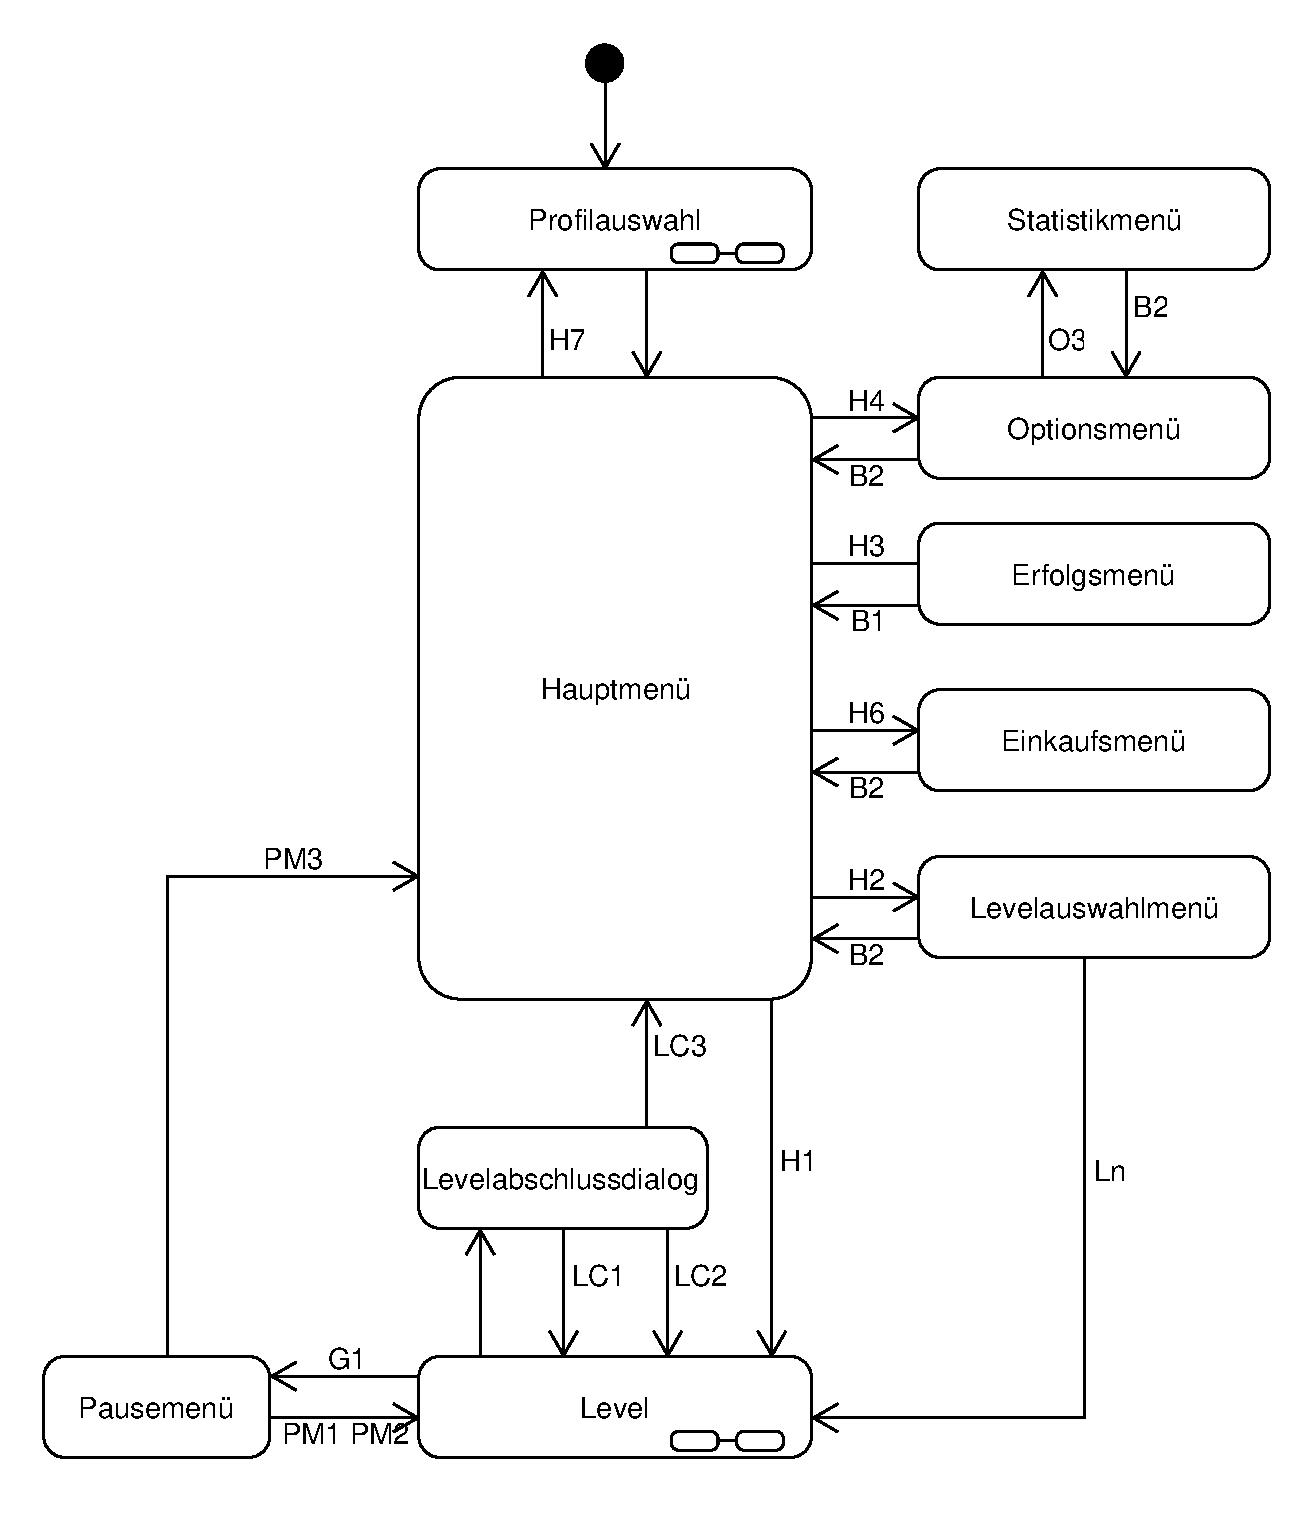
\includegraphics[scale=0.4]{../system_models/dynamic_models/menu_state_machine.pdf}
\caption{Zustandsautomat zur Menübedienung}
\end{figure}
%\restoregeometry

\begin{figure}[H]
\centering
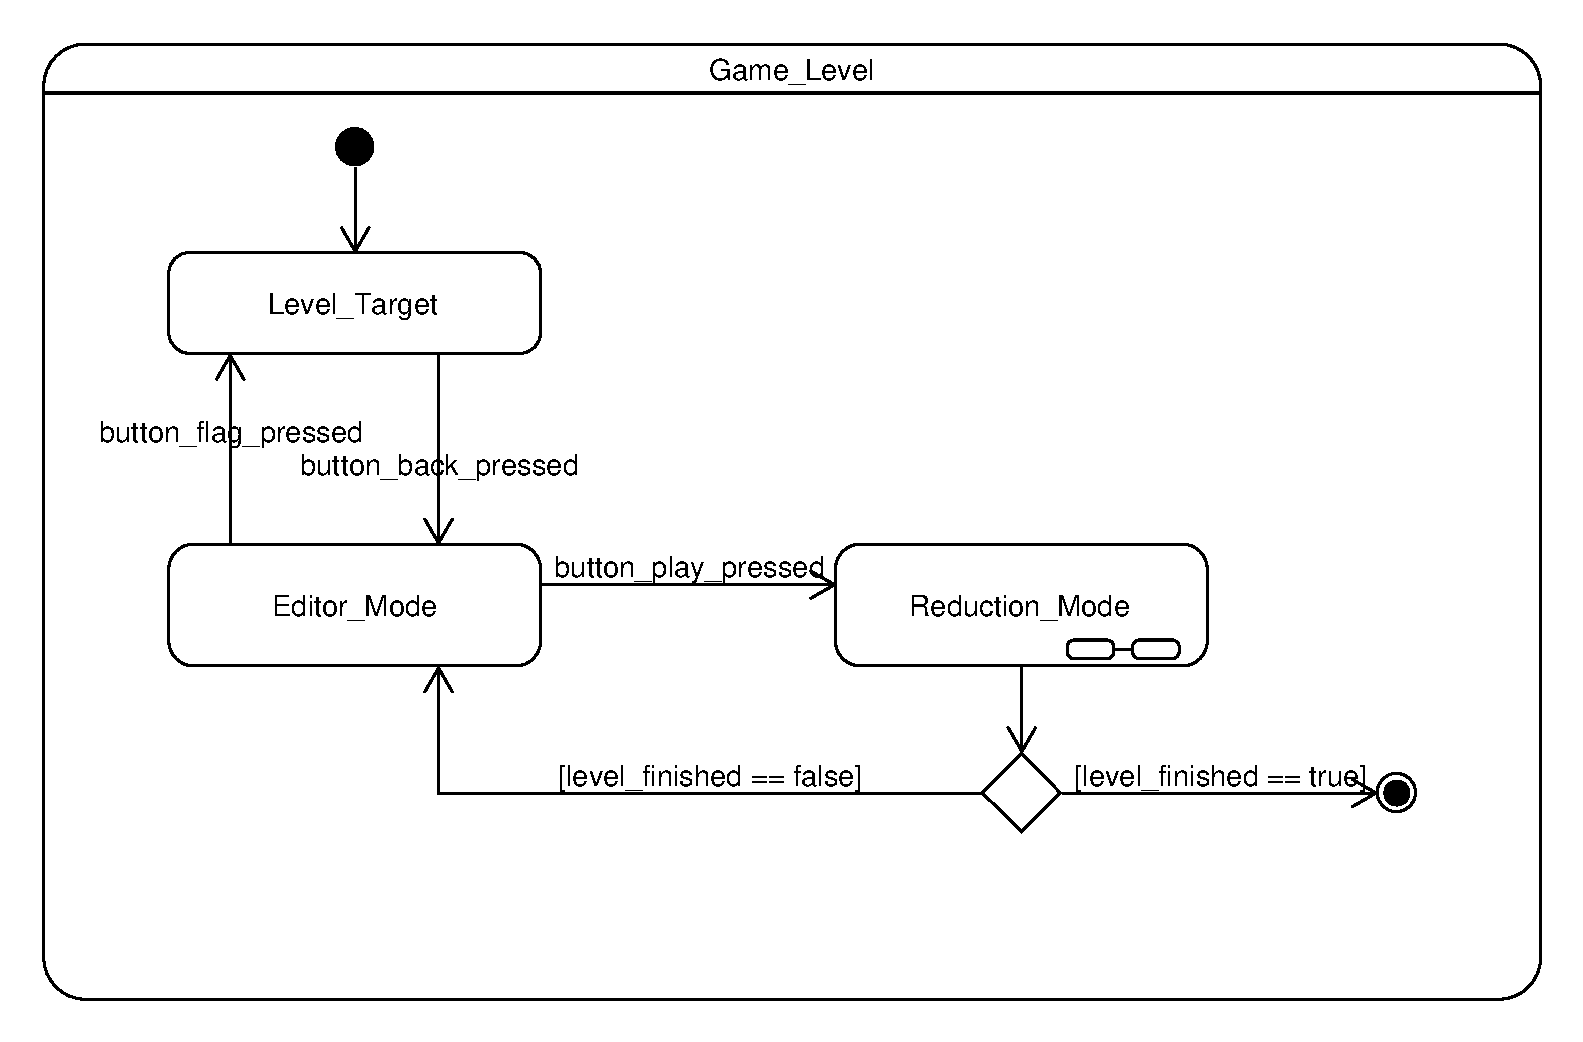
\includegraphics[scale=0.55]{../system_models/dynamic_models/game_level_state_machine.pdf}
\caption{Zustandsautomat zum Ablauf eines Levels}
\end{figure}

\begin{figure}[H]
\centering
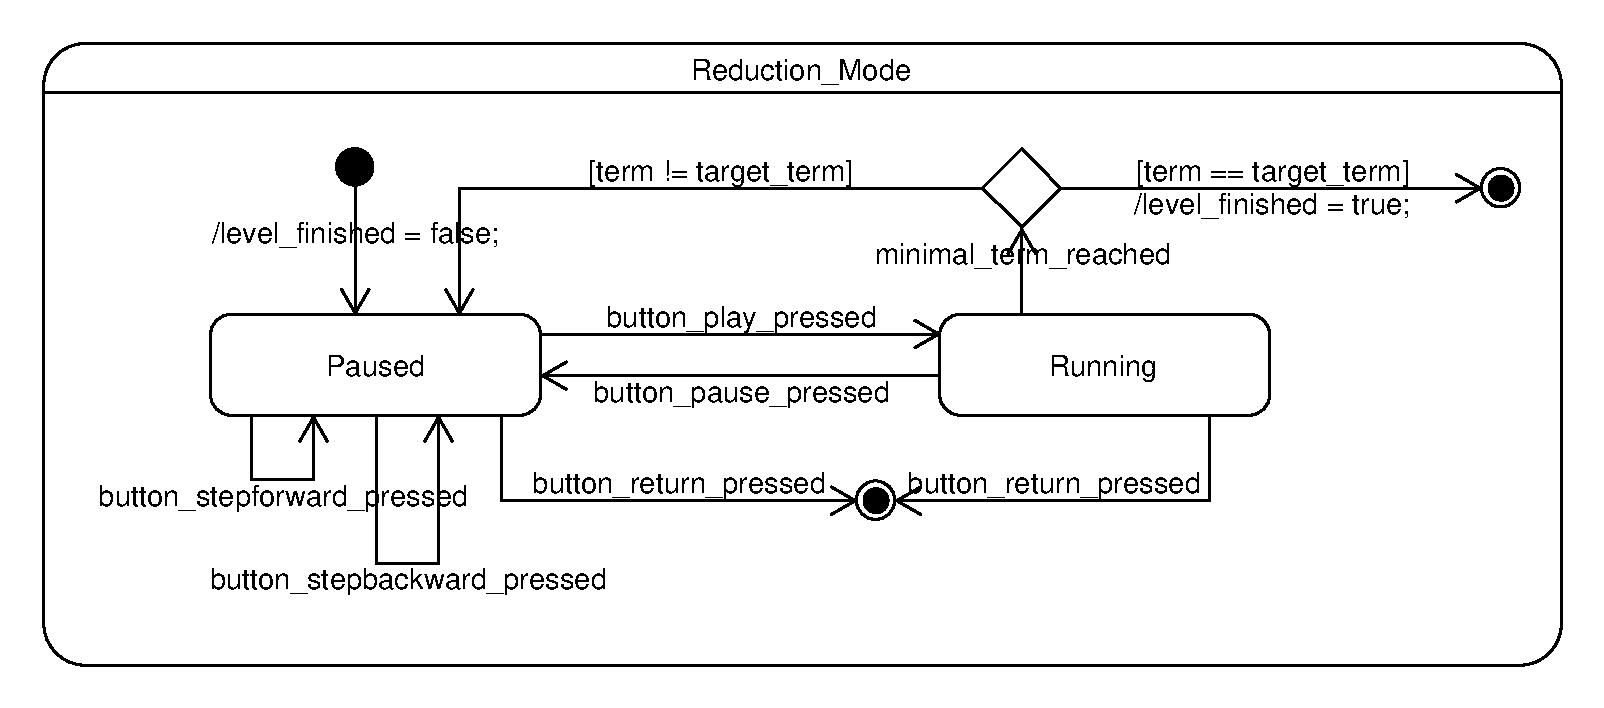
\includegraphics[scale=0.55]{../system_models/dynamic_models/reduction_mode_state_machine.pdf}
\caption{Zustandsautomat zur Funktion des Reduktions-Modus}
\end{figure}

\subsection{Benutzerschnittstelle}

GUI